\section*{Introdução}
\addcontentsline{toc}{section}{Introdução}
\hspace{13pt} A busca por um melhor entendimento dos processos e dinâmicas ocorridas na paisagem passa necessariamente por uma melhor compreensão do tempo \citep{gregory85}. 
Os avanços na utilização de séries temporais ao longo das últimas décadas vem contribuindo para o avanço da detecção de supressões florestais, sejam as relacionadas a processos antrópicos, como a processos naturais. Estes esforços são importantes principalmente
quando utilizados como subsídio ao desenvolvimento e a aplicação de políticas públicas conservacionistas. As aplicações podem ser vistas tanto em análises pontuais como em programas de monitoramento, assim como aplicadas em diversas escalas, mostrando sua flexibilidade para o subsídio de projetos locais \citep{rs12111815}, regionais \citep{Vancutsemeabe1603, silva_junior_brazilian_2021, brandt_unexpectedly_2020}, nacionais \citep{rs12111790} e até mesmo globais \citep{Hansen850, crowther_mapping_2015, POTAPOV2021112165}. A produção desses insumos contribuem diretamente, por exemplo, para o desenvolvimento de cooperações internacionais viáveis que foquem em políticas compensatórias visando a redução dos efeitos da mudança climática. 

No entanto, detectar mudanças na paisagem comparando mapas de uso e cobertura a partir de classificações prévias, tende a propagar erros e terem custo de produção elevado, como o caso de projetos governamentais como o realizado pelo IBGE \citep{ibge2020} ou projetos independentes como o Mapbiomas \citep{Souza2019}. O aumento na disponibilidade de imagens prontas para processamento  \citep{rs12030426} em plataformas como o Google Earth Engine facilitaram a aplicação de abordagens que buscam diminuir custos e facilitar o desenvolvimento de produtos no qual o foco pode estar compreendido no entendimento dos processos, sejam eles de curta ou de longa duração.

Ao longo dos últimos 10 anos algumas soluções passaram a ser desenvolvidas com o intuito de suprir esta demanda. Algoritmos de detecção de mudança em séries temporais como o Landtrendr foram desenvolvidos e aplicados inicialmente em ambientes de florestas temperadas \citep{KENNEDY2012117}. Desde as primeiras versões do algoritmo até hoje, muitas aplicações foram desenvolvidas em diversas áreas como: distúrbios florestais \citep{rs9050479, rs12223720}, mudanças em áreas urbanas \citep{rs12182883, rs13132438}, distúrbios causados por incêndios \citep{rs12091499, rs12233942}, mineração \citep{rs12101612, rs12142235}, distúrbios em áreas de proteção \citep{rs13091800}, detecção de mudanças ou abandonos de áreas de produção agrícola \citep{YIN201812, rs11101234, KOLECKA2021112340, DARA201849}, entre outros.

Alguns trabalhos em âmbito nacional também foram realizados e buscaram aplicar o algoritmo em áreas tropicais com o objetivo de entender seu comportamento em ambientes de maior diversidade ecológica. No entanto, todos os trabalhos focaram em contextos locais ou espacialmente limitados já que só puderam utilizar a primeira versão do algoritmo, ainda desenvolvido em linguagem proprietária IDL e com processamento exclusivo em ambiente offline, o que limitou significativamente a aplicação do mesmo para áreas extensas. O algoritmo foi aplicado primeiramente em áreas de várzea na floresta amazônica \citep{FRAGAL2016} e depois no contexto de Mata Atlântica em escala municipal \citep{Zebende2020} e estadual \citep{Weckmuller2019}. A partir da implementação do algoritmo na plataforma Google Earth Engine \citep{Kennedy2018}, a utilização do mesmo pode ser democratizada e possivelmente ampliada para extensões de terra maiores ao mesmo tempo que diminui o custo de produção do mapeamento, já que todo o processamento pesado passou a ser feito de forma gratuita e centralizada em um servidor online.

A partir de sua nova implementação surgiram possibilidades de aplicação do algoritmo visando a detecção de mudanças baseadas em trajetórias não só para paisagens locais como para grandes extensões. No entanto, para que sua aplicação seja de fato difundida como ferramenta de suporte à trabalhos de grande escala e que tenham significância para a elaboração de políticas nacionais e regionais, seria necessário entender seu desempenho quando aplicado a um grande grupo de ecossistemas e diferentes fitofisionomias.

Após análise de diferentes possibilidades de aplicação e áreas de estudo, verificou-se que o bioma Mata Atlântica poderia ser uma excelente e importante área de estudo para buscar o melhor entendimento da técnica proposta. Assim como sua extensão, o bioma possui outros números impressionantes. É na Mata Atlântica onde cerca de 100 milhões de pessoas vivem e também onde 70\% do produto interno bruto brasileiro é gerado, o que em parte explica o fato de hoje apenas cerca de 12\% de sua cobertura natural ter persistido e apenas 30\% dessas serem protegida em unidades de conservação. Apesar da baixa porcentagem de cobertura natural, é o bioma que abriga mais de 15.700 espécies de plantas e mais de 2.200 espécies de vertebrados registrados pela ciência (260-300 mamíferos; 930-990 aves; 200-300 répteis; 370-480 anfíbios; 300-350 peixes). As estimativas variam, mas, de qualquer forma, impressiona que a Mata Atlântica, representando apenas 0.8\% da superfície terrestre do planeta, abrigue cerca de 5\% das espécies de vertebrados e 5\% da flora mundial \citep{scarano2014}. Mesmo tratando-se do bioma brasileiro mais estudado, ainda há muito por descobrir. Entre 1990 e 2006, foram registradas mais de 1.190 novas espécies de plantas na Mata Atlântica, no coração da área urbana da cidade do Rio de Janeiro e novas espécies são encontradas com alguma frequência. Parte expressiva da fauna e da flora da Mata Atlântica é endêmica, ou seja, não ocorre em nenhum outro lugar do planeta. Estima-se que entre 43\% e 45\% do total de espécies de plantas e vertebrados sejam restritas a esse bioma \citep{scarano2014}.

A Mata Atlântica ainda apresenta a maior diferença altitudinal e latitudinal dentro todos os biomas brasileiros, o que justifica toda sua complexidade biológica, fitofisionômica e geomorfológica. Sendo assim, quando falamos de floresta no contexto da Mata Atlântica, não estamos falando de apenas uma floresta, mas de muitas. O bioma possui majoritariamente vegetação estacional semidecidual (403 mil km2), seguido por grandes áreas de vegetação ombrófila densa (183 mil km2) e ombrófila mista (160 mil km2). Além disso, possui também outros tipos de fitofisionomias como áreas estacionais deciduais, áreas de vegetação de estepe, savana, áreas de mangue, entre outros. 

Sendo assim, a análise se deu em áreas com vegetação de floresta. Foram excluídas áreas de floresta plantada, florestas em ambientes urbanos e também vegetação de mangue ou qualquer outra fitofisionomia não relacionada a tipos de vegetação de grande porte. O trabalho focou especialmente na análise e na validação de áreas de floresta ombrófila e estacional por serem as fitofisionomias mais predominantes no bioma.

O foco foi gerar tanto cenários de perda de vegetação quanto de ganho ao longo do período de 34 anos (1985 - 2018) com o intuito de entender melhor o comportamento do algoritmo na detecção de mudanças em um bioma tão complexo quanto a Mata Atlântica. 

\begin{figure}[h!]
    \centering
    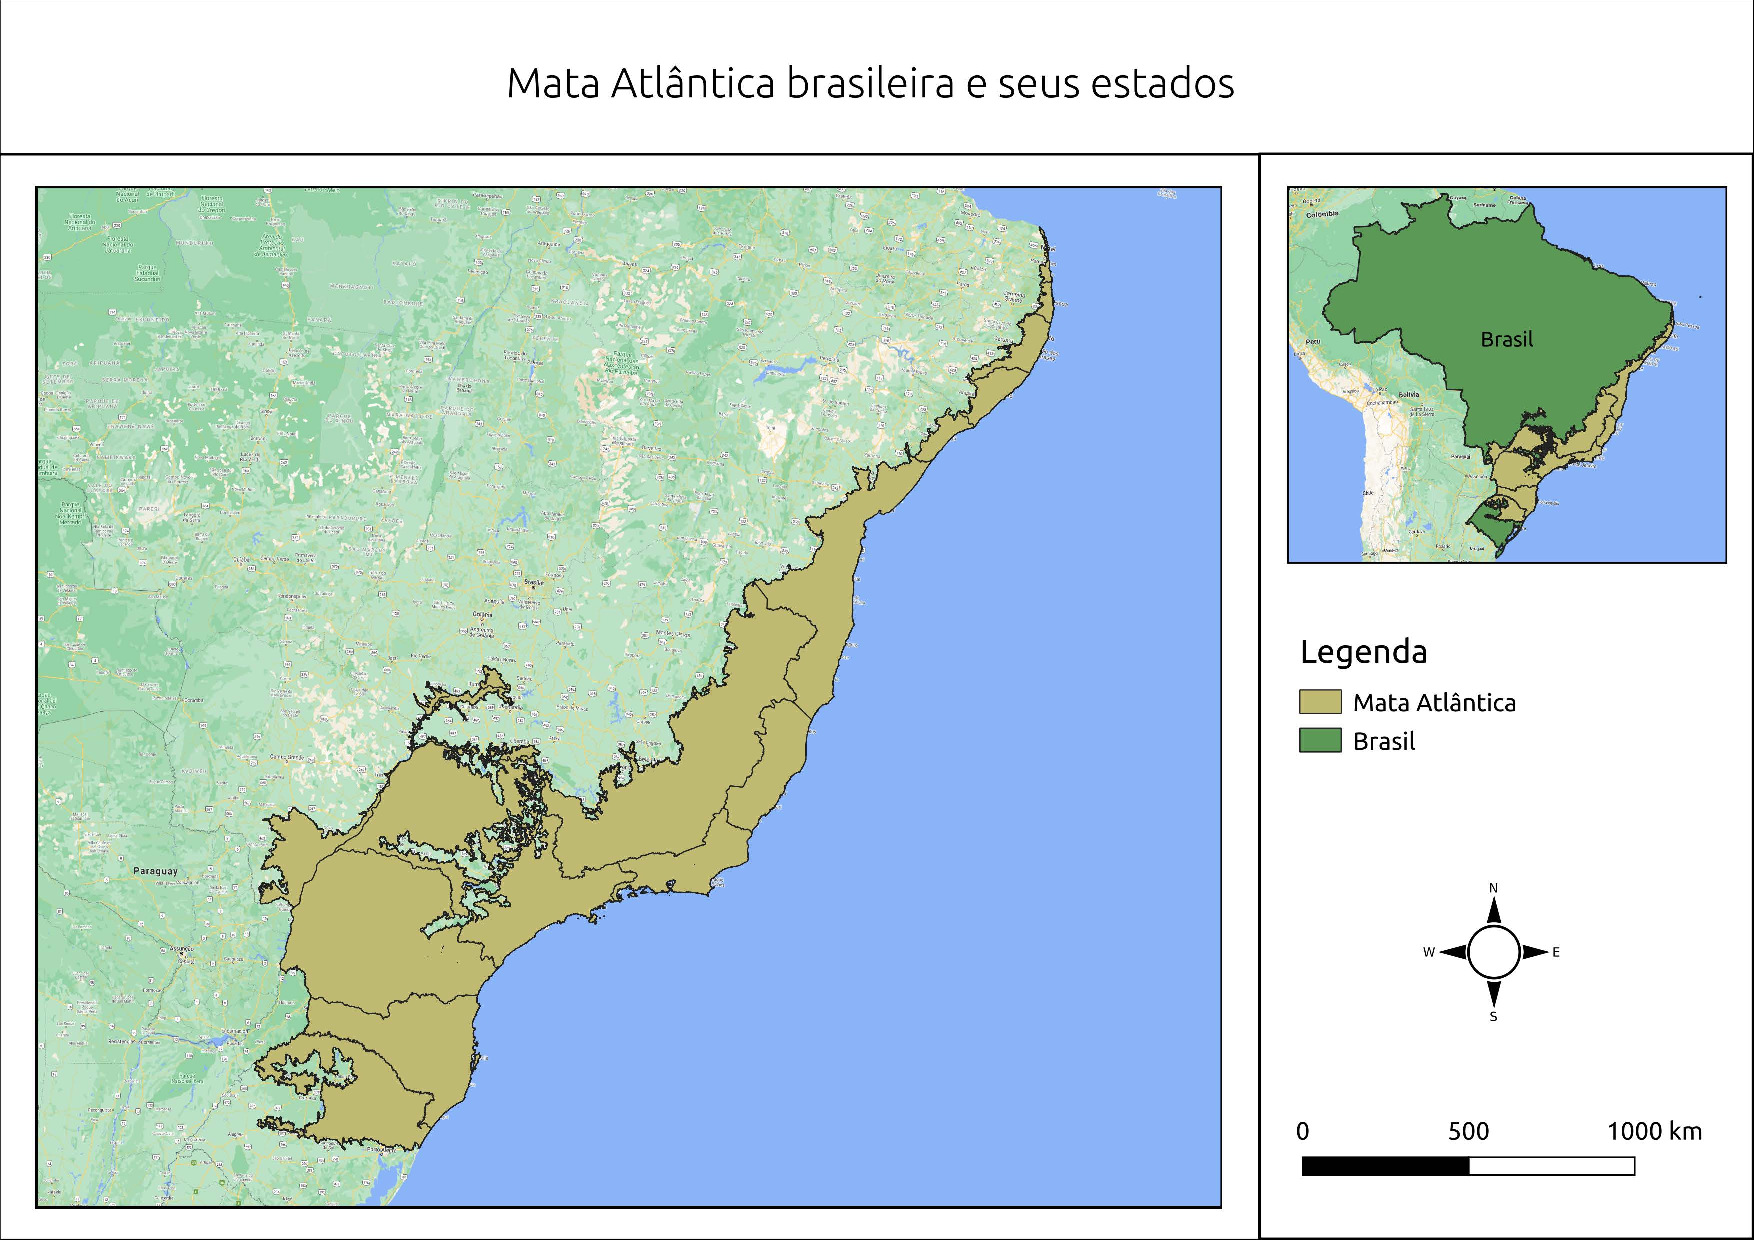
\includegraphics[scale=.5]{images/mata_atlantica.pdf}
    \caption{Área de Estudo - Mata Atlântica}
    \label{fig:mata_atlantica}
\end{figure}

\newpage

\subsection*{Questionamentos motivadores}
\addcontentsline{toc}{subsection}{Questionamentos motivadores}
Os questionamentos motivadores da pesquisa foram:
\begin{itemize}
    \item Como um algoritmo como o Landtrendr, inicialmente desenvolvido e utilizado para detecção de mudanças em ambientes de floresta temperada poderia ser utilizado para identificar mudanças ocorridas em uma paisagem complexa como a presente na Mata Atlântica? 
    
    \item Uma metodologia baseada na utilização do algoritmo conseguiria boa performance geral considerando as diferentes fitofisionomias presentes na Mata Atlântica?
    
    \item Como se distribuem as perdas e os ganhos de floresta no bioma ao longo das últimas três décadas? 
    
    % \item Como as unidades de conservação existentes da Mata Atlântica se comportaram ao longo dos anos? (ex. Parque Nacional da Serra da Bocaina, Parque Nacional da Serra dos Órgãos, etc)
\end{itemize}

\subsection*{Objetivos Gerais}
\addcontentsline{toc}{subsection}{Objetivos Gerais}
\hspace{13pt}  A tese tem como objetivo geral a análise da evolução do uso das áreas ocupadas por floresta no bioma da Mata Atlântica utilizando o algoritmo Landtrendr com o intuito de desenvolver e apresentar soluções metodológicas para o mapeamento de áreas tropicais de alta complexidade como a do bioma em questão.

\subsection*{Objetivos Específicos}
\addcontentsline{toc}{subsection}{Objetivos Específicos}
\begin{enumerate}

    \item Estruturação de uma metodologia para análise de mudanças em áreas de floresta tropical
    
    \begin{itemize}
        \item Definição do período, seleção das imagens e criação da composição da série temporal Landsat a ser utilizada;
        
        \item Estruturação de um fluxo de trabalho ótimo para o processamento dos dados através do desenvolvimento de software com objetivo de garantir a replicabilidade dos processos;
        
        % \item Compatibilização das imagens utilizadas de acordo com características geométricas e radiométricas com o intuito de evitar possíveis ruídos;
    \end{itemize}
    
    \item Detecção das mudanças através do mapeamento e classificação das trajetórias
    
    \begin{itemize}
        \item Definição dos parâmetros e do índice espectral para a execução do processo de segmentação temporal utilizando o algoritmo Landtrendr;
        
        \item Desenvolvimento do código na plataforma Google Earth Engine para a execução do algoritmo em todas as cenas que englobam o bioma da Mata Atlântica brasileira;
        
        \item Mapeamento das trajetórias florestais compatíveis com a escala 1:100.000 através da criação de mapas de detecção de magnitude, ano de início da mudança, duração e taxa de mudança;
        
        \item Avaliação da acurácia dos produtos gerados. Avaliar o desempenho do algoritmo em ambientes de florestas tropicais com alto nível de complexidade ecológica.
    \end{itemize}
    
    \item Análise da distribuição das mudanças no bioma da Mata Atlântica no período de 1985 até 2018
    
    \begin{itemize}
        \item Análise qualitativa através da criação de mapas de calor;
    \end{itemize}

    \begin{itemize}
        \item Conversão dos dados matriciais gerados em dados vetoriais com intuito de identificar áreas com maior nível de ocorrência de perdas e ganhos de acordo com divisões políticas e geoecológicas;
    \end{itemize}

\end{enumerate}